\chapter{非均匀流场中的光传输特性研究}
光是一种电磁波,物理学中存在大量关于电磁波在介质中传播特性的研究,这些研究表明光在介质中的传播过程呈现较强的波动性,麦克斯韦的衍射理论正是研究光波的传播的非常有利的工具,以场论为基础,建立电磁场中电场、磁场的微分关系,经过简化消元后,能够推导出非均匀介质中光传播的波动方程,如式\eqref{eq:maxwell}所示。
\begin{equation}
\begin{cases}
\nabla^2\mathbf{E}-\dfrac{\varepsilon\mu}{c^2}\cdot\dfrac{\partial^2\mathbf{E}}{\partial t^2}+\dfrac{\nabla\mu}{\mu}(\nabla\times\mathbf{E})+\nabla\big[\mathbf{E}\cdot\dfrac{\nabla\varepsilon}{\varepsilon}\big]=0\\
\nabla^2\mathbf{H}-\dfrac{\varepsilon\mu}{c^2}\cdot\dfrac{\partial^2\mathbf{H}}{\partial t^2}+\dfrac{\nabla\varepsilon}{\varepsilon}(\nabla\times\mathbf{H})+\nabla\big[\mathbf{H}\cdot\dfrac{\nabla\mu}{\mu}\big]=0
\end{cases}
\label{eq:maxwell}
\end{equation}
式中,$c=3\times10^8m/s$是真空中光速,为,$\mathbf{E},\mathbf{H}$为电磁场的电场及磁场,$\varepsilon,\mu$为相对介电常数及相对磁导率,绝大多数物质的介电常数$\varepsilon>1$,而对一般气体来说,相对磁导率$\mu=1$。

假设光在介质中的传播速度为$v$,那么物质的折射率$n$是由光在真空中与介质中的速度之比来定义的,即$n=c/v$。而光在介质中的传播速度又与该介质的相对磁导率、相对介电常数有简单关系:$v=c/\sqrt{\varepsilon\cdot\mu}$。联立两式,可以很快得到折射率与相对磁导率、相对介电常数的关系:
\begin{equation}
n=\sqrt{\varepsilon\cdot\mu}
\end{equation}

在研究湍流的气动光学效应时,流场的折射率$n$是与位置有关的函数,如果考虑通过流场的光波是波长为$\lambda$单色波,并且波函数$\mathbf{U}$与时间有$exp(-jwt)$的依赖关系,$w$为频率,由于流场的尺度$\Lambda$远远大于波长$\lambda$,可以将后两个偏振项近似为0,对方程\eqref{eq:maxwell}进行化简,可以得到简洁的波动方程:
\begin{equation}
\nabla^2\mathbf{U}-\frac{n^2}{c^2}\cdot\frac{\partial^2\mathbf{U}}{\partial t^2}=0
\label{eq:guangbodong}
\end{equation}
式中,$\mathbf{U}$是光波矢量,$n$为折射率。

对方程\eqref{eq:guangbodong}描述了光波在介质中的传输过程,对方程的求解能够精确描述流场对光传输的影响,但是波动方程很难得到解析解,并且由于飞行器周围流场由层流及湍流构成,流场结构非常复杂,使折射率随机变化,大大加大方程求解难度,目前工程上对气动光学效应研究的方法一般可以分为光线追迹方法、物理光学方法、波动光学方法以及统计光学方法这四类\cite{sutton1994}。

光线追迹方法主要是通过光线折射的原理,对从目标发出的每一条光线进行追踪,由不同光线在像平面的形成的点集合可以得到流场对光波传输的影响,该方法简单易行,但是由于采用了几何光学近似方法,无法确定传输特性与波长的关系,不能给出流场对光学传输特性的全面描述。

物理光学方法首先计算光波通过流场后的相位差分布,对其进行傅里叶变换求解相平面振幅分布,从而可以反推出流场的点扩散函数及调制传递函数,因此只要求解出光瞳函数,物理光学方法能比较全面地给出流场对光传输的影响。

波动光学的方法主要是利用子波原理,按照整体波面传播,计算传输到下一波面的过程,可以离散求解,最后得到波面像差,计算精度很高,但是折射率的随机分布使计算过程非常复杂,目前难以解决。

统计光学法将流场的变化看成具有一定特征的随机过程,利用概率论及随机过程结合实验数据,统计分析光波在流场中的传播特性,该方法可用于计算湍流脉动部分对光传输的影响。

实际工程共可以结合这几种研究方法进行综合考虑,将层流流场看作不随时间变化的非均匀流场,可以通过光线追迹及物理光学方法来求解层流流场的光传输特性,而对于具有随机性的湍流流场,可以引入流场“冻结”概念,对不同时刻的流场使用统计光学方法来描述。
\section{光线追迹理论及方法}
由于光在传输过程中呈现较强的波动性,导致在通过尺寸较小的空隙时会产生衍射现象,但是如果波长$\lambda$无限趋近于0,就消除了衍射情况,可以认为将光分为了无限多的细光线,光线就确定了光的能量传输走向,而在通常情况下,光学仪器尺寸远远大于光波长,这时可以忽略波长,光线追迹理论就是基于此假设。本文研究的光传输距离较短,且流场的湍流尺度远大于光波长,因此可以应用光线追迹法来进行研究。
\subsection{光线传输理论及基本方程}
费马原理直观地描述了光线的传播理论,该原理指出在所有可能的传输路径中,光线通过所需时间最少的就是那条唯一的传播路径,即光程。光线的光程是介质折射率$n$与光线通过实际路径的乘积,如果折射率随空间位置变化,光线从A传输到B的光程,可用折射率对路径积分来表示光程:
\begin{equation}
L_{OPL}=\int\limits_{A\to B}\!\!\!n\mathrm{d}s
\label{eq:guangcheng}
\end{equation}
式中,$n$为折射率。光程公式同时应该满足费马原理:$\partial\!\!\!\int\limits_{A\to B}\!\!\!n\mathrm{d}s=0$。

从式\eqref{eq:guangcheng}可以看出,在非均匀流场中,由于折射率的变化,光线的传输路径应该为曲线。为了求出光线在非均匀介质中的精确传输路径,一般可以利用正弦折射定律推导求出非均匀场中的光线传输基本方程,为了进行基础研究,可以假设非均匀介质在传播方向上连续分层,折射率呈现梯度分布,如图\ref{fig:guangxianchuanshu}所示,光线向x方向传播时,以$\theta_i$角度进入第$i$层折射率分界面,根据正弦折射定律,折射角应满足$n_1\sin\theta_1=n_2\sin\theta_2=n_3\sin\theta_3=\cdots=\text{常数}$,则$n_i\sin\theta_i=n_1\sin\theta_1$。
\begin{figure}[bhtp]
\centering
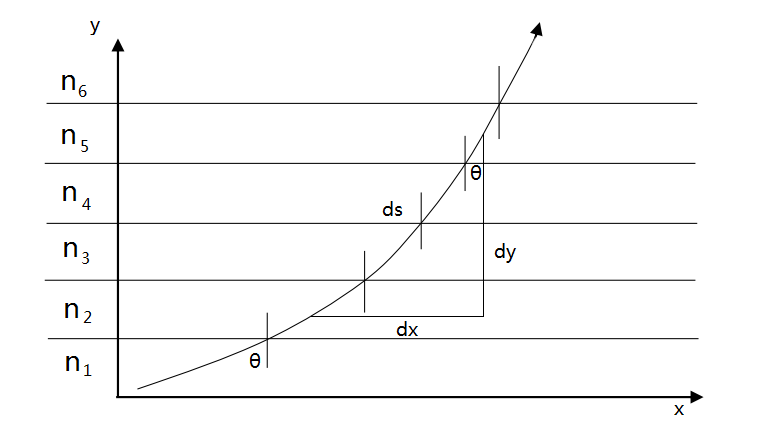
\includegraphics[width=0.5\linewidth]{guangxianchuanbo.PNG}
\caption{在非均匀连续分层介质中的光线传输}
\label{fig:guangxianchuanshu}
\end{figure}

当折射率连续变化,光线传输路径将变成一条连续的曲线,令$ds$表示表示光传输路径上的一小段弧长,则$(\mathrm{d}s)^2=(\mathrm{d}y)^2+(\mathrm{d}x)^2$,从图\ref{fig:guangxianchuanshu}可以看出$\mathrm{d}x/\mathrm{d}s=\sin\theta$,整合化简后,可以得到公式\eqref{eq:feijunyungl}。
\begin{equation}
\big(\frac{\mathrm{d}y}{\mathrm{d}z}\big)^2=\frac{n^2(y)}{n_1^2\sin^2\theta_1}-1
\label{eq:feijunyungl}
\end{equation}

该公式描述了在折射率分布确定情况下纵坐标随传输距离的变化,也就给出了光线的传播路径,如果对$x$微分,就能将光线传播方程化简,给出偏微分方程。
\begin{equation}
\frac{\mathrm{
d}^2y}{\mathrm{d}x^2}=\frac{1}{2n_1^2\sin^2\theta_1}\cdot\frac{\mathrm{d}n^2(y)}{\mathrm{d}y}
\label{eq:feijunyunglp}
\end{equation}

公式\eqref{eq:feijunyunglp}可以证明在均匀介质中,折射率$n(y)$是常数,等式右边为0,即$\mathrm{d}y/\mathrm{d}x^2=0$,表示光路是传播距离的一次函数,光线以直线传播,而在非均匀介质中,折射率的梯度变化导致光线以曲线形态传输,如果已知折射率分布及相应坐标,给出初始入射角,理论上就可以求解得到光传输路径,这就是光线传输的基本方程。

当考虑光线传输偏折,进一步分析光传输路径时,结合正弦折射定律,在介质折射率是连续且呈梯度变化的情况下,光线传输时会向着折射率较高的区域偏折,并且偏折角度大小应该与光路长度和折射率的梯度大小,同时如果折射率在平行于光传输方向有梯度变化时,并不会改变光走向,仅仅会改变光程大小。

由于光程可以说是光线在介质中所有可能路径的最小值,因此如果我们对公式\eqref{eq:guangcheng}应用费马原理,即光程的偏导数为零,这是一个变积分,可以用欧拉-拉格朗日方程表示,并且如果将光束入射方向定为x方向,进行消元化简后,可以得到如下方程组:
\begin{equation}
\left\{
\begin{aligned}
\frac{{\rm d}^2y}{{\rm d}x^2}=\Big[1+\Big(\frac{{\rm d} y}{{\rm d}x}\Big)^2+\Big(\frac{{\rm d}z}{{\rm d}x}\Big)^2\Big]\cdot
\Big[\frac{1}{n}\Big(\frac{\partial n}{\partial y}-\frac{{\rm d}y}{{\rm d}x}\cdot\frac{\partial n}{\partial x}\Big)\Big]\\
\frac{{\rm d}^2z}{{\rm d}x^2}=\Big[1+\Big(\frac{{\rm d} y}{{\rm d}x}\Big)^2+\Big(\frac{{\rm d}z}{{\rm d}x}\Big)^2\Big]\cdot
\Big[\frac{1}{n}\Big(\frac{\partial n}{\partial z}-\frac{{\rm d}z}{{\rm d}x}\cdot\frac{\partial n}{\partial x}\Big)\Big]
\end{aligned}\right.
\label{eq:feijunyunchuanshu}
\end{equation}
式中,$\dfrac{{\rm d}y}{{\rm d}x},\dfrac{{\rm d}z}{{\rm d}x}$表示入射光线的斜率,如果光束入射方向与坐标轴x平行,则有$\dfrac{{\rm d}y}{{\rm d}x}=\dfrac{{\rm d}z}{{\rm d}x}=0$,其他情况下入射光的斜率应均不等于零。对方程组\eqref{eq:feijunyunchuanshu}进行积分就可以得到光线在非均匀介质中的传输路径,但是这种非线性问题比较难以求解,在具体结合流场求解时,可以根据网格来离散化求解。
\subsection{光程差及偏折角理论}
介质折射率与光线在介质中的几何路径的乘积就是光线的光程(Optical Path Length),如果假定光束沿着z方向传输,折射率经过介质的传输路径为$\text{OPL}(x,y,z,t)$,由定义可以知道光线传输的光程公式为式\eqref{eq:opl}。
\begin{equation}
\text{OPL}(x,y,t)=\int_{0}^{L}n(x,y,z,t)\text{d}z
\label{eq:opl}
\end{equation}
式中,由于考虑湍流的随机运动,引入了流场随时间变化,$n(x,y,z,t)$为流场在$t$时刻$(x,y,z)$处的折射率值。由于光速非常快,光线经过流场的时间很短,流场一般来不及发生变化,因此可以考虑流场冻结的方法,认为流场结构在光线经过时不发生改变。

在折射率不同的介质中传输时,光波传输的速度不同,由于频率不发生变化,波长也就不同,令真空中光速为$c$,波长为$\lambda$,介质中光速为$u$,波长为$\lambda_i$,则介质折射率可以由速度或者波长比值来表示,$n=c/u=\lambda/\lambda_i$。如果光线的传输路径为$s$,则波长数为$s\lambda_i$,可以推导出,在介质中的波长数与光程上的绝对波长数相同,即:$s/\lambda_i=s\cdot n/\lambda$。则光线传输路程上的相位变化为:$\phi=(2\pi/\lambda)\cdot\text{OPL}$。那么两条初始相位差为$\phi_0$的光线经过流场后的相位差则为:$\Delta\phi=(2\pi/\lambda)\cdot(\text{OPL}_1-\text{OPL}_2)+\phi_0$。

为了方便讨论,并且考虑到波面计算等问题,我们可以引入光程差(Optical Path Difference)的概念,即两束光在介质中经过一定传输距离后的光程之差,我们在本文定义流场中的光程差为折射率起伏与相应传输距离的乘积,如公式\eqref{eq:opd},在气动光学中,光线传输距离可以近似为流场厚度,因此折射率的起伏决定了光程差的大小。
\begin{equation}
\text{OPD}(x,y)=\int_{0}^{L}\Delta n(x,y,z)\text{d}z
\label{eq:opd}
\end{equation}
式中,$\Delta n(x,y,z)$为流场当前位置的折射率与流场平均折射率之差。

前文讨论到光线在不均匀介质中的传输路径应该为曲线,那么,当光线出射时,会有一个偏折角$\theta$,如果将光线的传输路径定义为$s$,根据正弦折射定律可以知道,偏折角的变化与折射率的梯度相同如公式\eqref{eq:opljiao}。
\begin{equation}
\text{d}\theta/\text{d}s=\nabla n
\label{eq:opljiao}
\end{equation}

光束沿z方向传播,偏折角在$x,y$方向上有$\theta_x,\theta_y$两个分量,由于本文考虑的产生气动光学效应的流场厚度较小,可以将传播路程$s$近似等于传播方向上的$z$坐标改变,可以得到偏折角计算公式\eqref{eq:pianzhejiao}。
\begin{equation}
\frac{\partial\theta_x}{\partial z}=\frac{\partial n}{\partial x}~;
~~~~\frac{\partial\theta_y}{\partial z}=\frac{\partial n}{\partial y}
\label{eq:pianzhejiao}
\end{equation}
式中,偏折角分量及总偏折角应满足$\theta_x^2+\theta_y^2=\theta^2$关系。

通过光束传播过程中产生的偏折角,我们可以计算由此导致的瞄准误差$\beta_{BSE}$,瞄准误差实际上可以作为像偏移的简单判断,它可以用采样时间过程中的偏折角平均值表示:
\begin{equation}
\beta_{BSE}=\frac{1}{M}\sum\limits_{i-1}^{M}\theta_i
\end{equation}
式中,$\theta_i$表示第$i$个时间步长产生的偏折角,$N$是采样样本个数。
\section{流场引起的光学畸变分析}
光束在经过非均匀流场时会产生像差,根据光束在传播过程中的波动性比较明显的结论,可以通过衍射角度来分析流场引起的光学畸变现象,同时可以进一步分析出流场折射率随机脉动起伏对光学成像的影响,最后应该考虑如何评价这些气动光学效应。
\subsection{基于衍射理论的像差分析}
光在传输过程中的波动性较为明显,尤其是光在通过尺寸较小的小孔传播时,可以用衍射方法来分析传播过程,衍射问题也是光学中最困难的问题之一,难以得到解析解,在求解过程中,通常需要对其进行近似处理。

通过对\eqref{eq:guangbodong}的求解,假设在真空中考虑,令孔径面积为$A_0$,波长为$\lambda$,$U(x_0,y_0,0)$为初平面上光场分布,距离初平面$Z$的接受面光场分布为$U(x,y,Z)$,则有式\eqref{eq:guangbodongjie}。
\begin{equation}
U(x,y,Z)=-\frac{i}{\lambda}\int\frac{U_0(x_0,y_0,0)\cdot e^{ikr}}{r}\cdot\text{d}A_0
\label{eq:guangbodongjie}
\end{equation}
式中,$r=Z-xx_0/Z-yy_0/Z$。

在光波传输过程中,可以利用频谱分析方法把光波的振幅随空间位置的变化关系转换到随空间频率的变换,例如在垂直$z$轴的截平面上,平面波振幅$U(x,y)$可以通过空间频率$(\nu_x,\nu_y)$表示,如公式\eqref{eq:fuliye}。
\begin{equation}
U(x,y)=\iint_{-\infty}^{+\infty}A(\nu_x,\nu_y)\cdot\text{exp}[i2\pi(\nu_xx+\nu_yy)]\text{d}\nu_x\text{d}\nu_y
\label{eq:fuliye}
\end{equation}
式中,$\text{exp}[i2\pi(\nu_xx+\nu_yy)]$称为相位因子。这种表示方法将空间任意点的振幅$U(x,y)$利用空间频率表示,$A(\nu_x,\nu_y)$表示任意一个频率$(\nu_x,\nu_y)$所占的比例,该公式把一个平面的光波分解为沿着空间不同方向传播的平面波,每个平面波对应着一组空间频率$(\nu_x,\nu_y)$,这个频域函数$A(\nu_x,\nu_y)$就叫做角谱。

利用角谱可以在频率层面表示光传输过程,而通过对\eqref{eq:fuliye}进行傅里叶逆变换可以得到角谱$A(\nu_x,\nu_y,z)$的传播公式,也就确立了光波传输过程,将角谱公式代入波动方程后,经过变换积分计算化简后,得到公式\eqref{eq:kongjingjiaopu}。
\begin{equation}
A(\nu_x,\nu_y,z)=A_0(\nu_x,\nu_y)\cdot\exp(ikz)\cdot\exp\big[-i\pi\lambda z(\nu_x^2+\nu_y^2)\big]
\label{eq:kongjingjiaopu}
\end{equation}
式中,令$H(\nu_x,\nu_y)=\exp(ikz)\cdot\exp\big[-i\pi\lambda z(\nu_x^2+\nu_y^2)\big]$就是在折射率为1的自由空间中的传递函数,只要求出初平面的角谱分布,再与传递函数$H(\nu_x,\nu_y)$相乘,通过傅里叶逆变换就可以得知在$z=$z平面处的振幅分布。

在直角坐标系中,光沿z轴方向传播,假设在初平面上光波表示为$U(x,y,0)$,经过传输距离$z$后,到达z$=z$平面的光波为$U(x,y,z)$,通过傅里叶变换就可以得到平面波的角谱衍射理论基本公式\eqref{eq:jiaopuyanshe}。
\begin{equation}
\begin{aligned}
U(x,y,z)=&\int\limits_{-\infty}^{+\infty}\!\int\limits_{-\infty}^{+\infty}U(x,y,0)\cdot\exp\big[\frac{i2\pi z}{\lambda}(1-\lambda^2\nu_x^2-\lambda^2\nu_y^2)^{1/2}\big]\cdot\\
&\exp\Big\{i2\pi\big[\nu_x(x-x_0)+\nu_y(y-y_0)\big]\Big\}\text{d}\nu_x\text{d}\nu_y\text{d}x_0\text{d}y_0
\end{aligned}
\label{eq:jiaopuyanshe}
\end{equation}

在紧靠着孔径的地方光场分布一般遵循几何光学的规律,与光学孔径形状类似,但随着传输距离的增加,光场会发生衍射,光斑将会扩散,光强分布发生了明显改变,我们把从产生衍射的区域到无穷远处称为菲涅尔衍射区域,如果传输距离较远,衍射图像扩散严重,光强减弱较多,我们把这个区域称为夫琅禾费衍射区或者远场衍射,相对应的较近的地方称为近场衍射,可以看出菲涅耳衍射区包含了夫琅禾费衍射区。

为了能够通过计算得到衍射图像,通常都需要进行适当的近似,若考虑观测衍射成像的平面距离小孔$z$远大于孔径尺度,并且观测z轴附近的衍射情况,可以对一些参数进行近似处理,可见公式\eqref{eq:feijinsi}。
\begin{equation}
(1-\lambda^2\nu_x^2-\lambda^2\nu_y^2)^{1/2}\approx1-\frac{\lambda^2}{2}(\nu_x^2+\nu_y^2)
\label{eq:feijinsi}
\end{equation}

利用公式\eqref{eq:feijinsi}化简公式\eqref{eq:jiaopuyanshe},由于初平面孔径外的光场为零,因此可以只对孔径内部平面进行积分,先完成$\nu_x,\nu_y$的积分,利用傅里叶变换关系后可以得到菲涅尔衍射公式\eqref{eq:feinieer}。
\begin{equation}
\begin{aligned}
U(x,y,z)=&\frac{\exp(ikz)}{i\lambda z}\cdot\exp\big[\frac{ik}{2z}(x^2+y^2)\big]\int\limits_{-\infty}^{+\infty}\int\limits_{-\infty}^{+\infty}U(x_0,y_0,0)\cdot\\
&\exp\big[\frac{ik}{2z}(x_0^2+y_0^2)\big]\cdot\exp\Big[\frac{-i2\pi}{\lambda z}(xx_0+yy_0)\Big]\text{d}x_0\text{d}y_0
\end{aligned}
\label{eq:feinieer}
\end{equation}

由于式\eqref{eq:feinieer}中的相位因子$\exp\big[\frac{ik}{2z}(x_0^2+y_0^2)\big]$加大了计算积分的难度,在此如果令$z\gg\dfrac{k}{2}(x_0^2+y_0^2)$,可以把二次的相位因子在孔径上的积分近似为1,这种对于传输距离的较远的近似称作夫琅禾费近似,化简后可以得到夫琅禾费衍射公式\eqref{eq:fulanghefei},可以观察到光场分布就是小孔孔径上光场的傅里叶变换。
\begin{equation}
\begin{aligned}
U(x,y,z)=&\frac{\exp(ikz)}{i\lambda z}\cdot\exp\big[\frac{ik}{2z}(x^2+y^2)\big]\int\limits_{-\infty}^{+\infty}\int\limits_{-\infty}^{+\infty}U(x_0,y_0,0)\cdot\\
&\exp\Big[\frac{-i2\pi}{\lambda z}(xx_0+yy_0)\Big]\text{d}x_0\text{d}y_0
\end{aligned}
\label{eq:fulanghefei}
\end{equation}

夫琅禾费的衍射积分公式对条件要求非常高,它要求传输距离$z$远远大于孔径尺寸,假设光波为单色波,波长$\lambda$为600nm,那么当孔径尺寸$\Omega=0.25$mm时,传输距离$z$应该大于1.6m,若孔径尺寸$\Omega=0.025$m,那么观察距离必须大于1.6km才行,因此需要在远处才能观察到夫琅禾费衍射现象。

在以上衍射公式计算过程中,忽略了折射率的随机变化,直接令折射率为1,没有引入流场的随机特性,而在实际操作中,需要考虑折射率脉动引起的相位变化,假设在初平面$z=0$上有一个初始相位$\phi(x_0,y_0)$,在从初平面到$z=Z$平面传播过程中,相位畸变$\phi(x_0,y_0)$会有一个叠加累计,见公式\eqref{eq:xiangweicha}。
\begin{equation}
\Delta\phi=\int_{0}^{Z}\Delta n(x_0,y_0,z)\text{d}z
\label{eq:xiangweicha}
\end{equation}
式中,$\Delta n(x_0,y_0,z)$是初平面一点到$z=Z$平面上对应点传输路径中的折射率脉动。

因此当光在折射率随机非均匀分布的介质中传输时,引入相位变化后,在传输距离为$z$处的菲涅尔衍射公式\eqref{eq:fresnel}及夫琅禾费衍射公式式\eqref{eq:fraunhofer},这种基于折射率分布的衍射公式可以用来分析非均匀介质中的光波传输特性。
\begin{numcases}{}
\begin{aligned}
U(x,y,z)=&\frac{\exp(ikz)}{i\lambda z}\int\limits_{-\infty}^{+\infty}\int\limits_{-\infty}^{+\infty}U(x_0,y_0,0)\cdot\exp(ik\Delta\phi)\cdot\\
&\exp\Big\{i\frac{k}{2z}\big[(x-x_0)^2+(y-y_0)^2\big]\Big\}\text{d}x_0\text{d}y_0
\label{eq:fresnel}
\end{aligned}
\\
\begin{aligned}
U(x,y,z)=&\frac{\exp(ikz)}{i\lambda z}\int\limits_{-\infty}^{+\infty}\int\limits_{-\infty}^{+\infty}U(x_0,y_0,0)\cdot\exp(ik\Delta\phi)\cdot\\
&\exp\Big[-i\frac{k}{z}(xx_0+yy_0)\Big]\text{d}x_0\text{d}y_0
\label{eq:fraunhofer}
\end{aligned}
\end{numcases}

上节提到偏折角也是一个光传输过程中的重要参量,显示了光线在非均匀介质中传输一段距离后与入射方向的偏离角度,当引入偏折角概念时,由于传输距离Z相对于孔径尺寸非常大,可以近似地令$\theta_{x}=x/\text{Z},\theta_{y}=y/\text{Z}$,同时波数$k$表示为$2\pi/\lambda$,可以得到存在相位变化时,远场衍射的光波强度分布,同时在平面上观测时,可以消去$\exp(ikz)$这一项,得到远场光强分布公式\eqref{eq:yanshejiao}。
\begin{equation}
\begin{aligned}
U(\theta_{x},\theta_{y})=&\frac{-i}{\lambda \text{Z}}\iint\limits_\Sigma U(x,y,0)\cdot\exp\Big[ik\int_{0}^{\text{Z}}\Delta n(x,y,z)\text{d}z\Big]\cdot\\
&\exp\big[-ik(x\theta_{x}+y\theta_{y})\big]\text{d}x\text{d}y
\end{aligned}
\label{eq:yanshejiao}
\end{equation}
式中,$\Sigma$表示小孔区域,由于在孔径外光强都为0,因此仅对孔径内区域积分。

在非均匀介质中,光束的强度在传输过程中会有一定减弱,我们可以通过上述的衍射公式得到衍射的光场,然后利用该分布计算出成像平面的光强分布,假设远场的偏折角分量为$(\theta_x,\theta_y)$,在像平面$z=Z$处的衍射光强分布\cite{qiong2013}可以由公式\eqref{eq:yansheqiangdu}得到。
\begin{equation}
\begin{aligned}
I(\theta_x,\theta_y)=&U\cdot U^*=\frac{1}{\lambda^2Z^2}\iiiint U(x,y)\cdot U(x',y')\cdot\\
&\exp\Big\{ik\Big[\int\Delta n(x,y,z)\text{d}z-\Delta n(x',y',z')\text{d}z'\Big]\Big\}\cdot\\
&\exp\big[-ik\theta_x(x'-x)\big]\exp\big[ik\theta_y(y'-y)\big]\text{d}x'\text{d}y'\text{d}x\text{d}y
\end{aligned}
\label{eq:yansheqiangdu}
\end{equation}
式中,$\exp\big\{ik\big[\int\Delta n(x,y,z)\text{d}z-\Delta n(x',y',z')\text{d}z'\big]\big\}$体现了随机介质对光强度的影响,可以利用折射率脉动随时间的高斯分布将其变形,如公式\eqref{eq:gaosifenbu}。
\begin{equation}
\exp\Big\{-\frac{1}{2}k^2<\Big[\int\Delta n(x,y,z)\text{d}z-\Delta n(x',y',z')\text{d}z'\Big]^2>\Big\}
\label{eq:gaosifenbu}
\end{equation}

令流场的积分尺度大小为$\Lambda$,通过坐标系变换,能够得到爱里衍射斑的散射损失系数$\alpha$,爱里斑的强度分布可以通过公式\eqref{eq:yansheqiangdu}得到。
\begin{equation}
\begin{cases}
I(\theta)=\dfrac{I_0D^2}{4R^2\theta^2}\cdot J_I^2\big(\dfrac{\pi D\theta}{\lambda}\big)\\
\alpha=2k^2<\Delta n^2>\cdot\Lambda
\end{cases}
\end{equation}
式中,$I_0$为初平面的光波强度,$D$为小孔直径,$\lambda$为单色波波长,$J_I$为I阶的Bessel函数。第I阶贝塞尔函数$J_I(x)$可以表示为式\eqref{eq:ibessel}。
\begin{equation}
J_I(x)=\sum\limits_{m=0}^{\infty}\frac{(-1)^m}{m!\Gamma(I+m+1)}\Big(\frac{x}{2}\Big)^{I+2m}~~~~~~I\geq0
\label{eq:ibessel}
\end{equation}
式中,当I为整数时,有$(n+m)!=\Gamma(I+m+1)$,代入式\eqref{eq:ibessel},可以得到整数阶的贝塞尔函数。
\begin{equation}
J_I(x)=\sum\limits_{m=0}^{\infty}\frac{(-1)^m}{m!(I+m)!}\Big(\frac{x}{2}\Big)^{I+2m}~~~~~~I=0,1,2,\ldots
\label{eq:nbessel}
\end{equation}

由此,可以知道经过衍射后爱里斑的强度相对于初始强度的比值就可以通过损失系数$\alpha$确定,如公式\eqref{eq:jianruoyinzi}。
\begin{equation}
<\frac{I}{I_0}>=\exp\Big[-2k^2\int<\Delta n^2>\cdot\Lambda\text{d}z\Big]
\label{eq:jianruoyinzi}
\end{equation}

通过强度的比值公式可以看出,光在随机非均匀介质中传输时的光束强度变化与折射率的变化有直接关系,只要知道流场每一点的折射率分布,就能了解光束传输过程中的能量改变。
\subsection{气动光学的评价方法与评价指标}
光波经过随机非均匀流场会产生的波像差,这时在衍射像中的最大强度一定比同等情况下没有像差的系统中爱里斑中心强度小,这种情况导致了能量分布的变化,瑞利在研究这个现象的过程中发现,在观测截面查看有像差光学系统对光强分布影响时,如果波阵面偏离高斯参考球面的距离小于$1/4$波长,中心能量损失小于$20\%$,这种情况下系统对光学成像质量的影响不大,在可接受范围内,这也成为评价光学系统的一个重要指标,称为瑞利判据。

事实上,在分析光波经过流场后发生的波面畸变时,可以将光瞳函数$f(x,y)$分解为振幅$A(x,y)$和相位$\phi(x,y)$表示,如公式\eqref{eq:guangtonghanshu}。
\begin{equation}
f(x,y)=A(x,y)\cdot e^{-i\phi(x,y)}
\label{eq:guangtonghanshu}
\end{equation}
式中,光束截面的振幅一般起伏不大,对光瞳函数影响不大,可以令$A(x,y)\equiv1$,而波面的相位$\phi$是研究波面畸变的重点。

若令离参考面为传输距离的球面上相位变化平均为$\overline{\phi(x,y)}$,每一个波面点(x,y)上,光的波面畸变表示为$\Delta\phi(x,y)$,则有$\Delta\phi(x,y)=\overline{\phi(x,y)}-\phi(x,y)$。通过相位差就可以计算波面均方差$\sigma_\phi^2$,从而描述波面畸变情况\cite{haris2004},考虑到波动参数可能会随着时间变化,可以取系统平均,去除时间的影响,得到均方差公式\eqref{eq:junfangcha}。
\begin{equation}
\begin{aligned}
\sigma_\phi^2&=<\overline{[\overline{\phi(x,y)}-\phi(x,y)]^2}>
=<\overline{\phi^2(x,y)}>-<\overline{\phi(x,y)}>^2\\
&=\sigma_0^2-(\bar{\sigma}^2+\overline{K^2})
\end{aligned}
\label{eq:junfangcha}
\end{equation}
式中,$\sigma_0^2=<\overline{\phi^2(x,y)}>,\bar{\sigma}^2=<\bar{\phi}^2>,\overline{K^2}=<K^2(x^2+y^2)>$,$x,y$相互独立,$K$为倾斜因子,也可以沿角度方向测量相位变化,即$\overline{\phi(x,y)}=\bar{\phi}+K(x\cos\theta+y\sin\theta)$。波面均方差是用来计算气动光学效应的重要参数,尤其是涉及到斯特列尔比及光学传递函数的计算。

如果初平面的光场分布函数为$U(x,y)$,在观测平面及像平面的光场分布为$U(x',y')$,光瞳函数为$f(\eta,\xi)$,传输距离为Z,那么根据惠更斯-菲涅尔原理,可以得到$U(x',y')$表达式\eqref{eq:guangchang}。
\begin{equation}
\begin{aligned}
U(x',y')=&\text{C}\cdot\iint\limits_\Sigma U(x,y)\cdot\exp\Big[-i\frac{k}{\text{Z}}(x\eta+y\xi)\Big]\text{d}x\text{d}y\times\\
&\iint\limits_\Sigma f(\eta,\xi)\cdot\exp\Big[-i\frac{k}{\text{Z}}(x'\eta'+y'\xi')\Big]\text{d}\eta\text{d}\xi
\end{aligned}
\label{eq:guangchang}
\end{equation}
式中,$\Sigma$为孔径区域,若初平面的光源为点,则第一项积分为1,可以看出,光波在像面的振幅类似于是通过瞳函数经过傅里叶变换得到的,进行合适的坐标变换后,选择合适的归一化系数C,可以得到点振幅扩散函数$ASF(x',y')$,如公式\eqref{eq:dianzhenfu}。
\begin{equation}
ASF(x',y')=\text{C}\cdot\iint\limits_\Sigma f(x,y)\exp\Big[-i\frac{k}{Z}(xx'+yy')\Big]\text{d}z\text{d}y
\label{eq:dianzhenfu}
\end{equation}

通过点振幅扩散函数可以得到点扩散函数$PSF(x',y')$,它描述了光强度在像平面的相对分布,光场的强度正比于振幅的平方,可以得到点扩散函数$PSF(x',y')$。
\begin{equation}
PSF(x',y')=ASF(x',y')\cdot ASF^*(x',y')
\label{eq:diankuosan}
\end{equation}
式中,$ASF^*$表示点振幅扩散函数$ASF$的共轭。同时点扩散函数描述的是光强的相对分布,应满足$\iint\limits_{-\infty}^{+\infty}PSF(x',y')=1$,点扩散函数也可以作为一个描述流场气动光学效应的参量。

事实上只要对点扩散函数进行傅里叶变换,就可以得到流场的光学传递函数$OTF(f_{x'},f_{y'})$,也就能够从空间频率角度描述光传输效应
,如公式\eqref{eq:guangxuechuandi}。
\begin{equation}
OTF(f_{x'},f_{y'})=\iint PSF(x',y')\cdot\exp\big[-i2\pi(f_{x'}x'+f_{y'}y')\big]\text{d}x'\text{d}y'
\label{eq:guangxuechuandi}
\end{equation}

可以看出点振幅扩散函数、点扩散函数以及光学传递函数通过光瞳函数联系在一起,只要求出光瞳函数,或者说求出光波经过流场的相位畸变情况,就能够描述光束的传播过程,了解流场产生的气动光学效应,并且对其进行校正。

能够用来描述气动光学效应,对流场进行评估的另一个指标是斯特列尔比(strehl),它表示为有像差的衍射光斑的最大亮度$I$与同等传输距离下没有像差的衍射光斑的最大亮度$I_0$的比值\cite{mark2013},若传输距离为Z,可以由公式\eqref{eq:strehl}表示。由于一般光斑中心亮度最大,因此又将其称为中心亮度判据,可以作为判断图像能否分辨的依据。
\begin{equation}
S_\text{Z}=I/I_0
\label{eq:strehl}
\end{equation}

斯特列尔比可以通过点波面误差、点扩散函数、光学传递函数、泽尼克圆多项式等多种方法计算,由于定义简单并且比较容易计算,这是一种目前比较常用的评估气动光学效应的方法。本文定义的像点光强$I$为这一点光场分布的模的平方,并且需要对时间取平均,在极坐标下,可以利用点扩散函数得到像点光强$I(Q_\phi)$。
\begin{equation}
I(Q_\phi)=\Big(\frac{Aa^2}{\lambda Z^2}\Big)^2\cdot\bigg\vert\int_0^1\int_0^{2\pi}\exp\Big\{i\big[k\phi-\nu\rho\cos(\theta-\psi)-\frac{1}{2}u\rho^2\big]\Big\}\rho\text{d}\rho\text{d}\theta\bigg\vert^2
\end{equation}
式中,令$u,\nu$为0,就能得到无像差时像点的最大光强$I(Q_0)$。因此斯特列尔比可以表示为公式\eqref{eq:strehldiankuosan}。
\begin{equation}
S_\text{Z}(Q)=\frac{I(Q_\phi)}{I(Q_0)}=\frac{1}{\pi^2}\cdot\bigg\vert\int_0^1\int_0^{2\pi}\exp\Big\{i\big[k\phi-\nu\rho\cos(\theta-\psi)-\frac{1}{2}u\rho^2\big]\Big\}\rho\text{d}\rho\text{d}\theta\bigg\vert^2
\label{eq:strehldiankuosan}
\end{equation}

根据统计光学原理,可以通过光学传递函数来表示中心光强的比值,通常情况下由于光学传函数在积分宽度上并不是均匀变化的,因此可以利用系统平均处理,假设系统总的光学传递函数为$f_0(x,y)$,通过波面均方差$\sigma_\phi^2$,结合光学传递函数,可以得到中心光强的比值,见公式\eqref{eq:strehlchuandi}。
\begin{equation}
\begin{aligned}
<I/I_0>&=\frac{4}{\pi}\iint\limits_{-\infty}^{+\infty}\exp(-k^2\sigma_\phi^2[1-r(x,y)])\cdot f_0(x,y)\text{d}x\text{d}y\\
&=\frac{4}{\pi}\exp(-k^2\sigma_\phi^2)\iint\limits_{-\infty}^{+\infty}\exp\big[k^2\sigma_\phi^2r(x,y)\big]\cdot f_0(x,y)\text{d}x\text{d}y
\end{aligned}
\label{eq:strehlchuandi}
\end{equation}
式中,$r(x,y)$为相位差$\Delta\phi$的相关系数。将指数部分用泰勒级数展开:
\begin{equation}
\exp\big[k^2\sigma_\phi^2r(x,y)\big]=\sum\limits_{n=0}^{\infty}\frac{(k^2\sigma_\phi^2)^n}{n!}\cdot r^n(x,y)
\end{equation}
上式代入\eqref{eq:strehlchuandi}后,对其进行近似处理,令孔径尺寸D远大于折射率脉动尺寸$l_x,l_y$,再通过级数展开,可以得到大孔径近似下的斯特列尔比,如公式\eqref{eq:streldakongjing}。
\begin{equation}
\begin{cases}
<I/I_0>\sim\exp(-k^2\sigma_\phi^2)\Big\{1+\dfrac{8\cdot F(k^2\sigma_\phi^2)}{(\text{D}/l_x)(\text{D}/l_y)}\Big\}\\
F(x)=\sum\limits_{n=1}^{\infty}\dfrac{x^n}{n^2\cdot n!}~~~~~~~~~~~(x=k^2\sigma_\phi^2)
\end{cases}
\label{eq:streldakongjing}
\end{equation}

可以将式\eqref{eq:streldakongjing}的光强比值分为两部分,第一部分为$\exp(-k^2\sigma_\phi^2)$影响衍射极限,削弱光强,第二部分则对分布更广更分散的光束产生影响,Hogge认为这种光束属于非相干光束,如果衍射孔径足够大,满足D>$6l_x$,就可以忽略第二项的影响。

公式\eqref{eq:junfangcha}给出了波阵面的相位均方差$\sigma_\phi^2$,在通过波面误差来计算斯特列尔比时,我们假设波像差的均方值在像差不大的情况下能够表示参考球面中心的光强,此时斯特列尔比能表示为公式\eqref{eq:strehljunfangcha}。
\begin{equation}
S_\text{Z}(Q)=e^{-k^2\cdot\sigma_\phi^2}
\label{eq:strehljunfangcha}
\end{equation}

对比公式\eqref{eq:streldakongjing}、\eqref{eq:strehljunfangcha},可以发现当作大孔径近似处理即令D$>6l_x$时,利用光学传递函数得到的斯特列尔比与直接利用波面相位均方差得到的结果一致。至此,可以发现只要能够给传输路径中空间每点的出折射率分布,就能利用点扩散函数来描述成像的模糊情况,用斯特列尔比来描述光强度的衰减,还可以利用偏折角来体现光学成像的偏移,利用光学传递函数(OTF)就可以得到像面光场分布,从而对气动光学效应进行评价,为进一步的光学校正提供基础。
\section{高速流场中的气动光学计算分析}
在飞行器高速飞行时,周围空气与其相互作用,会形成复杂的湍流流场,对于流场的光学特性研究,可以将其分为平均流场及随机脉动流场两种情况分别分析,平均流场主要依据光线追迹理论,对光程差、传输方程等进行计算,而湍流部分主要依据统计学理论进行分析。一般对光束经过流场前后的畸变进行分析时,可以计算通过流场作用后的光波再经过光学透镜成像,从而对其进行气动光学效应的具体分析,其成像机理如图\ref{fig:qidongguangxuejisuanjili}。

\begin{figure}[bhtp]
\centering
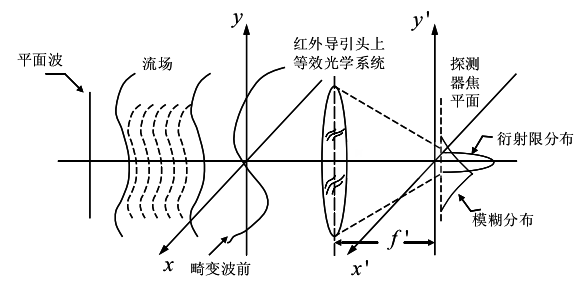
\includegraphics[width=0.8\linewidth]{qidongguangxuejili.PNG}
\caption{光束经过流场后的计算分析图}
\label{fig:qidongguangxuejisuanjili}
\end{figure}
\subsection{平均流场的光传输计算}
飞行器外的流场随飞行过程不断变化,不具有空间、时间不变性,无法应用线性光学的理论描述,但是抛开流场随机脉动部分,考虑稳定的层流部分时,由于这部分的流场比较稳定,可以认为不随时间变化。层流流场的密度在空间上呈现不均匀分布,对其气动光学效应分析时,可以利用光线追迹法得到光在流场中的传输路径,从而了解光程差、相位差等参数。

在通过光线追迹法计算具体流场的光程差时,一般先通过计算流体力学的相关知识得到流场中的密度、温度、压强等物理参量,继而通过这些参数来计算流场的诸如波面畸变、点扩散函数等气动光学效应。由于对流场的模拟一般会将三维区域划分成多个小单元构成的网格结构,因此在计算光程差时,可以通过计算每个小单元中的光程差然后累加得到,如公式\eqref{eq:lisanguagnchengcha}。
\begin{equation}
L_{OPD}=\sum\limits_{i=1}^{N}\Delta n_i\cdot\Delta l_i
\label{eq:lisanguagnchengcha}
\end{equation}
式中,$\Delta n_i$为第$i$个单元中心的折射率与平均流场的折射率之差,$\Delta l_i$为光线经过第$i$个单元上下表面的实际路程。

这样通过网格单元离散单元的光程差进行叠加后就可以得到光束穿过整个流场区域的光程差,如果定义光波波数$k=2\pi/\lambda$,将波数与光程差相乘就能够得到光束的相位差,也就能够分析光束波面畸变情况。

平均流场对光束传输产生的像偏移可以通过偏折角来快速、直观地表示,通过\eqref{eq:pianzhejiao},结合光程差概念,假设光束沿z方向进入流场,那么就可以计算出光束在像面沿$x,y$方向的偏折角$\theta_x,\theta_y$,如公式\eqref{eq:pingjunpianzhejiao}。
\begin{equation}
\left\{
\begin{aligned}
\theta_x&=\frac{\partial L_{OPD}}{\partial x}=\frac{\partial}{\partial x}\int_0^L\Delta n(x,y,z){\rm d}z\\
\theta_y&=\frac{\partial L_{OPD}}{\partial y}=\frac{\partial}{\partial y}\int_0^L\Delta n(x,y,z){\rm d}z
\end{aligned}
\right.\label{eq:pingjunpianzhejiao}
\end{equation}

通过偏移角来衡量光斑相对中心的偏移主要基于流场折射率的起伏来得到,而折射率主要通过流场来影响,因此需要经过大量计算才能得到精确结果,而事实上当我们需要快速直观地对飞行器周围流场进行大致像偏移的评估时,可以根据一些流场已知参数直接判断。如果我们知道了来流速度或者飞行器飞行速度$u$,给出飞行器头部的半锥角$\alpha$,可以通过式\eqref{eq:jibojiao}知道头部激波角$\theta$。
\begin{equation}
\tan\alpha=\frac{(u\sin\theta)^2-1}{\Big(\dfrac{\gamma+1}{2}u^2-\sin^2\theta+1\Big)\tan\theta}
\label{eq:jibojiao}
\end{equation}
式中,$\gamma$为流场气体的比热比。

令G-D系数为$K_{\rm GD}$,$\beta$为入射光线与飞行器中轴的夹角,$\rho_0,\rho_1$分别为远场密度以及激波后的密度,$\delta$为像偏移角,通过这些基本参数就可以得到大致像偏移情况。
\begin{equation}
\left\{
\begin{aligned}
\frac{\cos(\theta+\beta)}{\cos(\theta+\beta+\delta)}=\frac{1+K_{\rm GD}\cdot\rho_1}{1+K_{\rm GD}\cdot\rho_0}\\
\rho_1=\rho_0\cdot\frac{(\gamma+1)u^2\sin^2\theta}{(\gamma-1)u^2\sin^2\theta+2}
\end{aligned}
\right.\label{eq:jibopianyi}
\end{equation}

公式\eqref{eq:jibojiao}及\eqref{eq:jibopianyi}联立,就能够通过飞行器本身结构参数、流场速度、远场的密度以及入射光线的入射角度四个已知的物理参量计算得到像偏移情况,这种方法在计算简单、方便的同时牺牲了一些精确度,没有通过流场内部结构来分析光束的传输,一般情况下,这种近似计算可以用来大致地快速分析流场产生的像偏移,对此有一个宏观上的判断。

在通过光线追迹法结合计算流体软件网格划分离散计算得到光线经过每个小单元格的光程差,累加后能得到穿过流场后每一点的全部光程差,如果假设光束穿过流场时的光程差分布为$P(x,y)$,并且忽略瞄准误差,那么对其作傅里叶变换,就可以得到焦平面上的光场分布,令小孔直径为D,$\theta_x,\theta_y$为孔径投射到像平面的角坐标,我们可以得到像面上的光场分布及光强分布如式\eqref{eq:guangchangfenbu}、\eqref{eq:guangqiangfenbu}。
\begin{align}
U(\theta_x,\theta_y)&=\bigg(\frac{4}{\pi\text{D}^2}\bigg)\cdot\int_{-\frac{\text{D}}{2}}^{\frac{\text{D}}{2}}\int_{-\sqrt{(\text{D}/2)^2-x^2}}^{\sqrt{(\text{D}/2)^2-x^2}} e^{-ikP(x,y)}\cdot e^{ik(\theta_x,\theta_y)}\text{d}x\text{d}y
\label{eq:guangchangfenbu}\\
I(\theta_x,\theta_y)&=\big|U(\theta_x,\theta_y)\big|^2
\label{eq:guangqiangfenbu}
\end{align}

因此如果能够计算出光学窗口处流场的光程差,就能得到时间上近似稳定的平均流场对光束传输的影响,可以通过定义光学孔径,同时忽略瞄准误差,采用二元的傅里叶变换的方法,就能计算出平面光经过流场后的光场分布情况。
\subsection{湍流流场的光传输计算}
在考虑湍流引起的光学传输特性变化时,由于湍流运动的随机性,可以通过统计特性来描述流场中空气的运动规律,通常情况下可以引入亚格子模型分析湍流折射率脉动,湍流的气动光学效应可以认为是沿着光传输方向的累加产生的。亚格子模型主要利用相关函数来描述密度脉动情况,一般可以采用冯$\cdot$卡门模型、高斯模型及指数模型三种,假设密度相关函数为$C(x,y,z)$。
\begin{align}
&\text{冯$\cdot$卡门模型:}
&C(x,y,z)&=\frac{2^{2/3}}{\Gamma(1/3)}(l_{xyz})^{1/6}\cdot B_{1/3}\big[(l_{xyz})^{1/2}\big]\\
&\text{高斯模型:}
&C(x,y,z)&=\exp[-l_{xyz}]\\
&\text{指数模型:}
&C(x,y,z)&=\exp\big[-(l_{xyz})^{1/2}\big]\label{eq:zhishuxiangguanxishu}
\end{align}
式中,$l_{xyz}=(x/l_x)^2+(y/l_y)^2+(z/l_z)^2$,$\Gamma(1/3)$是Gamma函数,$B_{1/3}\big[(l_{xyz})^{1/2}\big]$是第二类修正Bessel函数。

波面的畸变可以通过折射率协方差来计算,如果假设均方差折射率脉动为$\overline{n'^2}$,湍流密度相关系数定为$C(x,y,z)$,可以得到折射率协方差公式。
\begin{equation}
R(x,y)=\int_0^\text{L}\int_{-\text{Z}}^{\text{L}-\text{Z}}\overline{n'^2}(x',y',z')\cdot C(x,y,z)\text{d}z\text{d}z'
\label{eq:zheshelvxiefangcha}
\end{equation}

通过以上公式,可以完整地表示沿传输方向的折射率变化,得到相位的方差、相关函数及相关长度。
\begin{align}
&\text{相位方差:}&\sigma_\phi^2=k^2\cdot R(0,0)\label{eq:xiangweifangcha} \\
&\text{相位相关函数:}&C_\phi(x,y)=k^2\cdot\phi(x,y) \\
&\text{相位相关尺度:}&l_\phi=\frac{1}{\sigma^2}\int_{-\infty}^{\infty}\int_{-\infty}^{\infty}C_\phi(x,y)\text{d}x\text{d}y \label{eq:xiangweixiangguanchangdu}
\end{align}

可以发现,湍流密度相关系数影响了相位变化的计算,相位方差可以利用相位相关长度与折射率脉动的均方差联合表示,取加权函数为1后,得到公式\eqref{eq:xiangweijunfangcha}
\begin{equation}
\sigma_\phi^2=2k^2\int_0^\text{L}\overline{n'^2}(z)l_\phi\text{d}z
\label{eq:xiangweijunfangcha}
\end{equation}

对相位相关函数进行傅里叶变换就可以得到湍流相位脉动功率谱,取$x,y$方向上的空间频率分别为$\nu_x,\nu_y$,相位脉动功率谱可以表示为\eqref{eq:xiangweimaidong}
\begin{equation}
F_\phi(\nu_x,\nu_y)=\frac{1}{(2\pi)^2}\int_{-\infty}^{\infty}\int_{-\infty}^{\infty}C_\phi(x,y)\cdot\exp[-i(\nu_xx+\nu_yy)]\text{d}x\text{dy}
\label{eq:xiangweimaidong}
\end{equation}

通过功率谱函数$F_\phi(\nu_x,\nu_y)$可以求出湍流介质中时间平均的调制传递函数$f_{MTF}(\nu_x.\nu_y)$,从而用亚格子模型描述了湍流对光传输路径的影响。
\begin{align}
&f_{MTF}(\nu_x,\nu_y)=\exp\big\{-\big[C_{\phi B}(0,0)-C_{\phi B}(\nu_x,\nu_y)\big]\big\}\\
&C_{\phi B}(\nu_x,\nu_y)=\int_{-\infty}^{\infty}\int_{-\infty}^{\infty}F_\phi(\nu_x,\nu_y)\cdot\exp\big[-i(\nu_xx+\nu_yy)\big]\text{d}x\text{d}y
\end{align}
式中,$C_{\phi B}(\nu_x,\nu_y)$为相位相关函数,与功率谱$F_\phi(\nu_x,\nu_y)$有关。

对于包含湍流流场的混合流场的气动光学效应,就可以利用光经过平均流场在焦平面所成像的点扩散函数PSF与相对应的调制传递函数$f_{MTF}$通过卷积得到像的强度分布$I$。
\begin{equation}
I\Big(\frac{x}{\lambda f},\frac{y}{\lambda f}\Big)=\mathscr{F}^{-1}\big\{f_{MTF}(\nu_x,\nu_y)\big\}*\mathscr{F}\Big\{PSF\big(\frac{x}{\lambda f},\frac{y}{\lambda f}\big)\Big\}
\end{equation}
式中,$f$为光瞳到焦平面距离即焦距,$\mathscr{F}$为傅里叶变换。

对于时间平均流场能够采用光线追迹法计算出光束的偏折角,而对于湍流脉动流场,可以通过偏折角的均方差来描述湍流场对光束的影响。在利用统计方法计算得到折射率均方差的基础上,通过下式得到偏折角均方差。
\begin{equation}
\overline{\Delta\theta^2}=-\overline{\Delta n^2}\cdot H\int_0^\infty\frac{1}{r^2}\cdot\frac{\rm d}{{\rm d}r}\Big(\frac{r^2{\rm d}C_n(\Delta x,\Delta y,\Delta z)}{{\rm d}r}\Big){\rm d}r
\end{equation}
式中,$C_n(\Delta x,\Delta y,\Delta z)$是折射率相关函数,可以选择不同的经验模型进行计算,$r=\sqrt{\Delta x^2+\Delta y^2+\Delta z^2}$,H为传输距离,在湍流场中的近距离传输下可以近似为流场厚度。

至此,利用光程差、偏折角等可以描述出时间平均流场对光传输的影响,通过偏折角均方差可以表述湍流部分对光传输特性的影响,利用光学传递函数能够描述出光束经过混合流场的光强分布情况,基于这些气动光学效应的描述、计算方法,为应用中的光学校正以及气动光学效应的削弱方法提供有力的理论基础和前期准备。
\section{本章小结}
本章主要阐述了光波在非均匀介质中的传输、衍射理论,讨论了非均匀介质引起的波面畸变现象,将流场对光传输的影响划分为平均流场及随机脉动流场分别作用后效果的叠加,推导了波前畸变计算公式,对斯特列尔比、点扩散函数、光学传递函数等光学评价指标进行了推导计算,并且研究了高速流场中如何对流场的稳定部分及随机部分的气动光学效应进行计算,在平均流场部分采用光线追迹法求解出平均波面畸变,在随机脉动部分引入亚格子模型,主要通过功率谱函数及光学传递函数来计算像面光强分布,描述光束传播过程。